% !TEX program = arara
% arara: pdflatex
% arara: biber
% arara: pdflatex
% arara: pdflatex
% arara: clean: { files: [ Bericht.out ] }
% arara: clean: { files: [ Bericht.aux, Bericht.bbl ] }
% arara: clean: { files: [ Bericht.bcf, Bericht.blg ] }
% arara: clean: { files: [ Bericht.log, Bericht.run.xml ] }
% arara: clean: { files: [ Bericht.toc, Bericht-blx.bib ] }
% 

\documentclass{Bericht}
\usepackage{todonotes}
\usepackage[utf8]{inputenc}
\usepackage{hyperref} % http://ctan.org/pkg/hyperref
\usepackage{graphicx}
%\usepackage[ngerman]{babel} % deutsche Silbentrennung
\hypersetup{
	colorlinks = true,
	linkcolor  = black
}

\begin{document}

\maketitle

% % % % %

\tableofcontents
\clearpage

\section{Einleitung}
	\todo[inline]{Autor: Kim}
Das Thema Zeitempfinden spielt in unserer modernisierten Gesellschaft eine immer wichtiger werdende Rolle. Zwischen Arbeit, Freizeit und Familie ist es wichtig, seine Zeit ganz genau zu planen und jede freie Minute auszunutzen. Aufgrund des Wissens, dass die arbeitende Bevölkerung sich an bestimmte Zeitregeln hält und versucht den Alltag optimal zu managen und unter Betrachtung der zunehmenden Relevanz von Zeitmanagement und Zeitsparen, richteten wir unsere Forschung auf das Thema der Zeitmanpulation. Zunächst gilt zu definieren, was Zeit überhaupt ist: „Zeit ist das Nacheinander von Zuständen und Ereignissen, die erlebbar und messbar sind. Sie ist eine physikalische Größe für die Vergänglichkeit und Veränderungen“. (\underline{http://definition-online.de/zeit/}) 
	\par
	In unserer Lebenswelt gibt es bestimmte Zeitgeber, von der Uhrzeit selber einmal abgesehen, die uns Hinweise geben, wieviel Zeit vergangen ist. Für uns galt es nun herauszufinden, ob es möglich ist, anhand gängiger Zeitgeber, die jeden einzelnen Menschen seit der Geburt täglich begleiten, eine Manipulation des Zeitempfindens auszulösen. Anhand unserer Forschungsfrage: „Kann man das Zeitempfinden in der Virtuellen Welt durch bestimmte Zeitgeber manipulieren“ erschufen wir eine Virtuelle Welt, durch die unsere späteren Probanden mit Hilfe einer VR-Brille manipulierte Zeitgeber erlebten. 
	\par
	 Wir legten einen weiteren Fokus unserer Arbeit auf die Zeitschätzung. Jeder Proband wurde gebeten, vor und nach dem Befinden in der Virtuellen Welt eine bestimmte Sekundenanzahl abzuschätzen, ohne auf Hilfsmittel zuzugreifen, wie beispielsweise eine Armbanduhr. Auf diese Weise wollen wir herausfinden, ob sich die Zeitschätzung vor dem Befinden in der Virtuellen Welt von der Zeitschätzung nach dem Befinden in der Virtuellen Welt unterscheidet.
Dieser Bericht führt über die Ideenfindung unserer Forschungsschwerpunktes zu unseren Hypothesen. Nach der technischen und kreativen Umsetzung unseres Experiments und unserer virtuellen Welt wird der detaillierte Ablauf des Experiments beschrieben. Im Zweiten Teil- dem empirischen Teil- folgen die Auswertungen, Ergebnisse und Interpretationen und der Bezug zu unseren Hypothesen. Am Ende des Berichts gibt es einen kurzen Überblick über die Zusammenarbeit der Forschungsgruppe und ein abschließendes Fazit. 
\par
 \textit{„Zeit ist das, was man an der Uhr abliest.“ ( Albert Einstein )}
 \par
  Ob diese Definition wirklich ausreicht, oder ob es andere wichtige Zeitgeber gibt, die das menschliche Zeitempfinden vorgeben, gilt es herauszufinden. 

\section{Ideenfindung}
	\todo[inline]{Autor: Berna}
	Hier steht die Ideenfindung.

\section{Hypothese}
	\todo[inline]{Autor: Berna}
		Hier steht die Hypothese.

\clearpage
\section{Verlauf}
	\todo[inline]{Autor: Marvin \& Daniel}
	\subsection{Planung/Recherche} % Marvin
	
%Erster Kontakt
Erster Berührungspunkt mit dem Bachelorprojekt ¡Experiment! war für viele Gruppenmitglieder die Vorstellung eben dessen durch Thorsten Kluß am 24.01.2017 an der Hochschule für Künste, bzw. deren Wiederholung am 06.04.2017 an der Universität Bremen. Erweitert wurde der zweite Termin dabei durch eine Führung der Räume des 'Cartesiums', sowie eine Beschreibung der vorangegangen Bachelorprojekte. Hierdurch konnte ein erster Eindruck über die verschiedenen Versuchsaufbauten und ferner der Beschaffenheit unseres Projekts gewonnen werden. An dieser Stelle wurde zunächst eine Recherche-Aufgabe zu vorbereiteten Texten ausgeteilt, welche allein oder in kleineren Gruppen bearbeitet und später präsentiert werden sollte.\\
\\
%Erwartungen
Am darauffolgenden Termin wurden uns von den Dozenten (Thorsten Kluß und Jaime Maldonaldo, später zusätzlich Kerstin Bub) alle Erwartungen, sowie Schein- und Arbeitsbedingungen dargelegt.\\
\\
%Social & Arbeitsweise/Zeiten
Neben den üblichen 'Kennenlern-Ritualen', wie z.B. dem Herausstellen der eignen Stärken und Schwächen anhand von 'Skill-Profilen', wurden die ersten zwei Wochen der Projektarbeit hauptsächlich für technische Organisation, Planungs- und Recherchezwecke genutzt. Dabei entschied man zunächst, dass ein 'Scrum'-Modell mit geteilter 'Scrum-Master'-Position für das Projektmanagement genutzt werden soll. Anhand der bereits erwähnten Fähigkeitenprofile wurde die Gruppe 7-3 in zwei Teams mit unterschiedlichen Schwerpunkten aufgeteilt('Design' und 'Organisation').\\
Weiterhin wurde ein umfassender Stundenplan aus den einzelnen Stundenplänen für das restliche Studium jedes Teilnehmers erstellt. Anhand dessen wurden Zeiten an vier Tagen der Woche ermittelt, welche für Treffen der Arbeitsgruppe zum Bachelorprojekt genutzt werden sollten, mit einem zusätzlich Slot am Donnerstag für ein Meeting mit den Dozenten. \\
Zu Beginn jeden Arbeitstages wurde ein 10-minütiges 'Scrum-Treffen' gehalten, in denen anstehende Aufgaben aus dem Backlog und Probleme besprochen wurden. Diese besonderen Treffen wurden jedoch nie regelmäßig eingehalten, vor allem in späteren, arbeitsintensiveren Phasen nicht.\\
Ferner wurde für die Protokollführung der Treffen eine feste Reihenfolge angelegt.\\
\\
%Raum
Leider war es unseren Dozenten nicht möglich, eine dedizierten Raum für unseren Arbeitsprozesse zu erhalten, weshalb die Treffen je nach Situation im Konferenzraum [x.x] des vierten Stockwerks oder den Räumen [x.x] und [x.x](ebenfalls vierter Stock) im Cartesium abgehalten worden sind. Um Zugang zu der Etage und diesen Räumen zu gewährleisten, erhielten wir mit einiger Verzögerung jedoch Türchips für das spezielle Schließsystem des Cartesiums.\\
\\
% Tech
Auch wurden alle technischen Lösungen zur Arbeitsweise in dieser Zeit implementiert. Als zentrale Sammelstelle für sämtliche Dokumente wurde ein Board beim Service 'Trello' genutzt. Dort ließen sich bequem und zugänglich für alle Teilnehmer sämtliche wöchentlichen Sprints sowie der Backlog des Scrum, die Protokolle und der Stundenplan, etc. ablegen. Für schnelle Kommunikation untereinander wurde der Nachrichtendienst 'WhatsApp' genutzt, da diese Applikation bereits auf sämtlichen Endgeräten der Teilnehmer installiert war. Leider wurde dieser Dienst nicht von den Dozenten genutzt und wir verließen uns auf Kommunikation per E-Mail mit diesen, sowie Telefonate in dringenden Fällen.\\
\\
%Recherche
Die ersten Rechercheleistungen beschäftigten sich hauptsächlich mit wissenschaftlichen Arbeitsweisen, existierenden technischen Möglichkeiten und bereits durchgeführter Forschung. Vollkommen fehlgeleitet und geblendet von technischen Besonderheiten wie dem möglichen Hand-Tracking durch 'LeapMotion' oder der Bewegungsteuerung durch [die Kugel] versuchten wie eine Forschungsfrage passend zu diesen zu entwickeln.\\
Wie im 'Paragraphen 2: Ideenfindung' beschrieben, dauerte es eine gewisse Zeit bis wir eine konkrete, realisierbare Forschungsfrage zur Manipulation des Zeitempfindens innerhalb der 'Virtual Reality' ausarbeiten konnten. Maßgeblich geholfen hat uns dabei die Grundlagenforschung zur Zeitwahrnehmung in der VR von Gerd Bruder.\\
\\
%Überschneidung
Die genauen Spezifikationen an unser Experiment gemäß der Forschungsfrage wurden nach Rücksprache mit den Dozenten immer wieder verändert. Hierdurch entstand viel unbenutzbares Material, da wir überschneidend bereits damit begonnen hatten, 3D-Objekte nach den ersten Anforderungen für unsere Versuchswelt zu erstellen. Dies geschah fälschlicherweise aus dem Versuch heraus, bereits verlorene Zeit aufzuholen, wodurch jedoch nur mehr 'Verschnitt' produziert worden ist, was uns ultimativ uns mehr Zeit gekostet hat.\\
\\
%Weiterführend
Wir approximierten, dass sich ab diesem Zeitpunkt unser Projekt in 3 Phasen (Programmierphase, Versuchsphase, Evaluation/Paper) 	unterteilen ließe und legten Deadlines für die einzelnen fest. Im Laufe des Projektes sollten wir jedoch erkennen, wie weit entfernt diese Einschätzungen von der Realität abwichen.

	\subsection{Design} % Daniel
		\todo{methodisches Versuchsdesign}
		Angefangen haben wir mit dem Erstellen von 3D-Objekten. Aus einer Liste mit benötigten Objekten suchte sich jeder aus dem Technikteam einige heraus und begann sie zu designen. Folgende Objekte wurden erstellt, wenn auch nicht alle im finalen Projekt zum Einsatz kamen:
		
		\begin{itemize}
			\setlength{\itemsep}{0em}
			\item Ampel
			\item Autos
			\item Blume
			\item Bäume
			\item Büsche
			\item Garten
			\item Gehsteige
			\item Heißluftballon
			\item Hund
			\item Häuser
			\item Laterne
			\item Menschliche NPCs
			\item Mülleimer
			\item Parkbank
			\item Plakat
			\item Rasenfläche
			\item Reiher
			\item Schaukel
			\item Sonne
			\item Straße
			\item Straßenschilder
			\item Supermarkt
			\item Wolken
			\item Zimmerpflanze (Kaktus)
		\end{itemize}
		
		\begin{figure}[!htbp] % here - top - bottom - page, das ! erzwingt die Position falls möglich
			\centering
			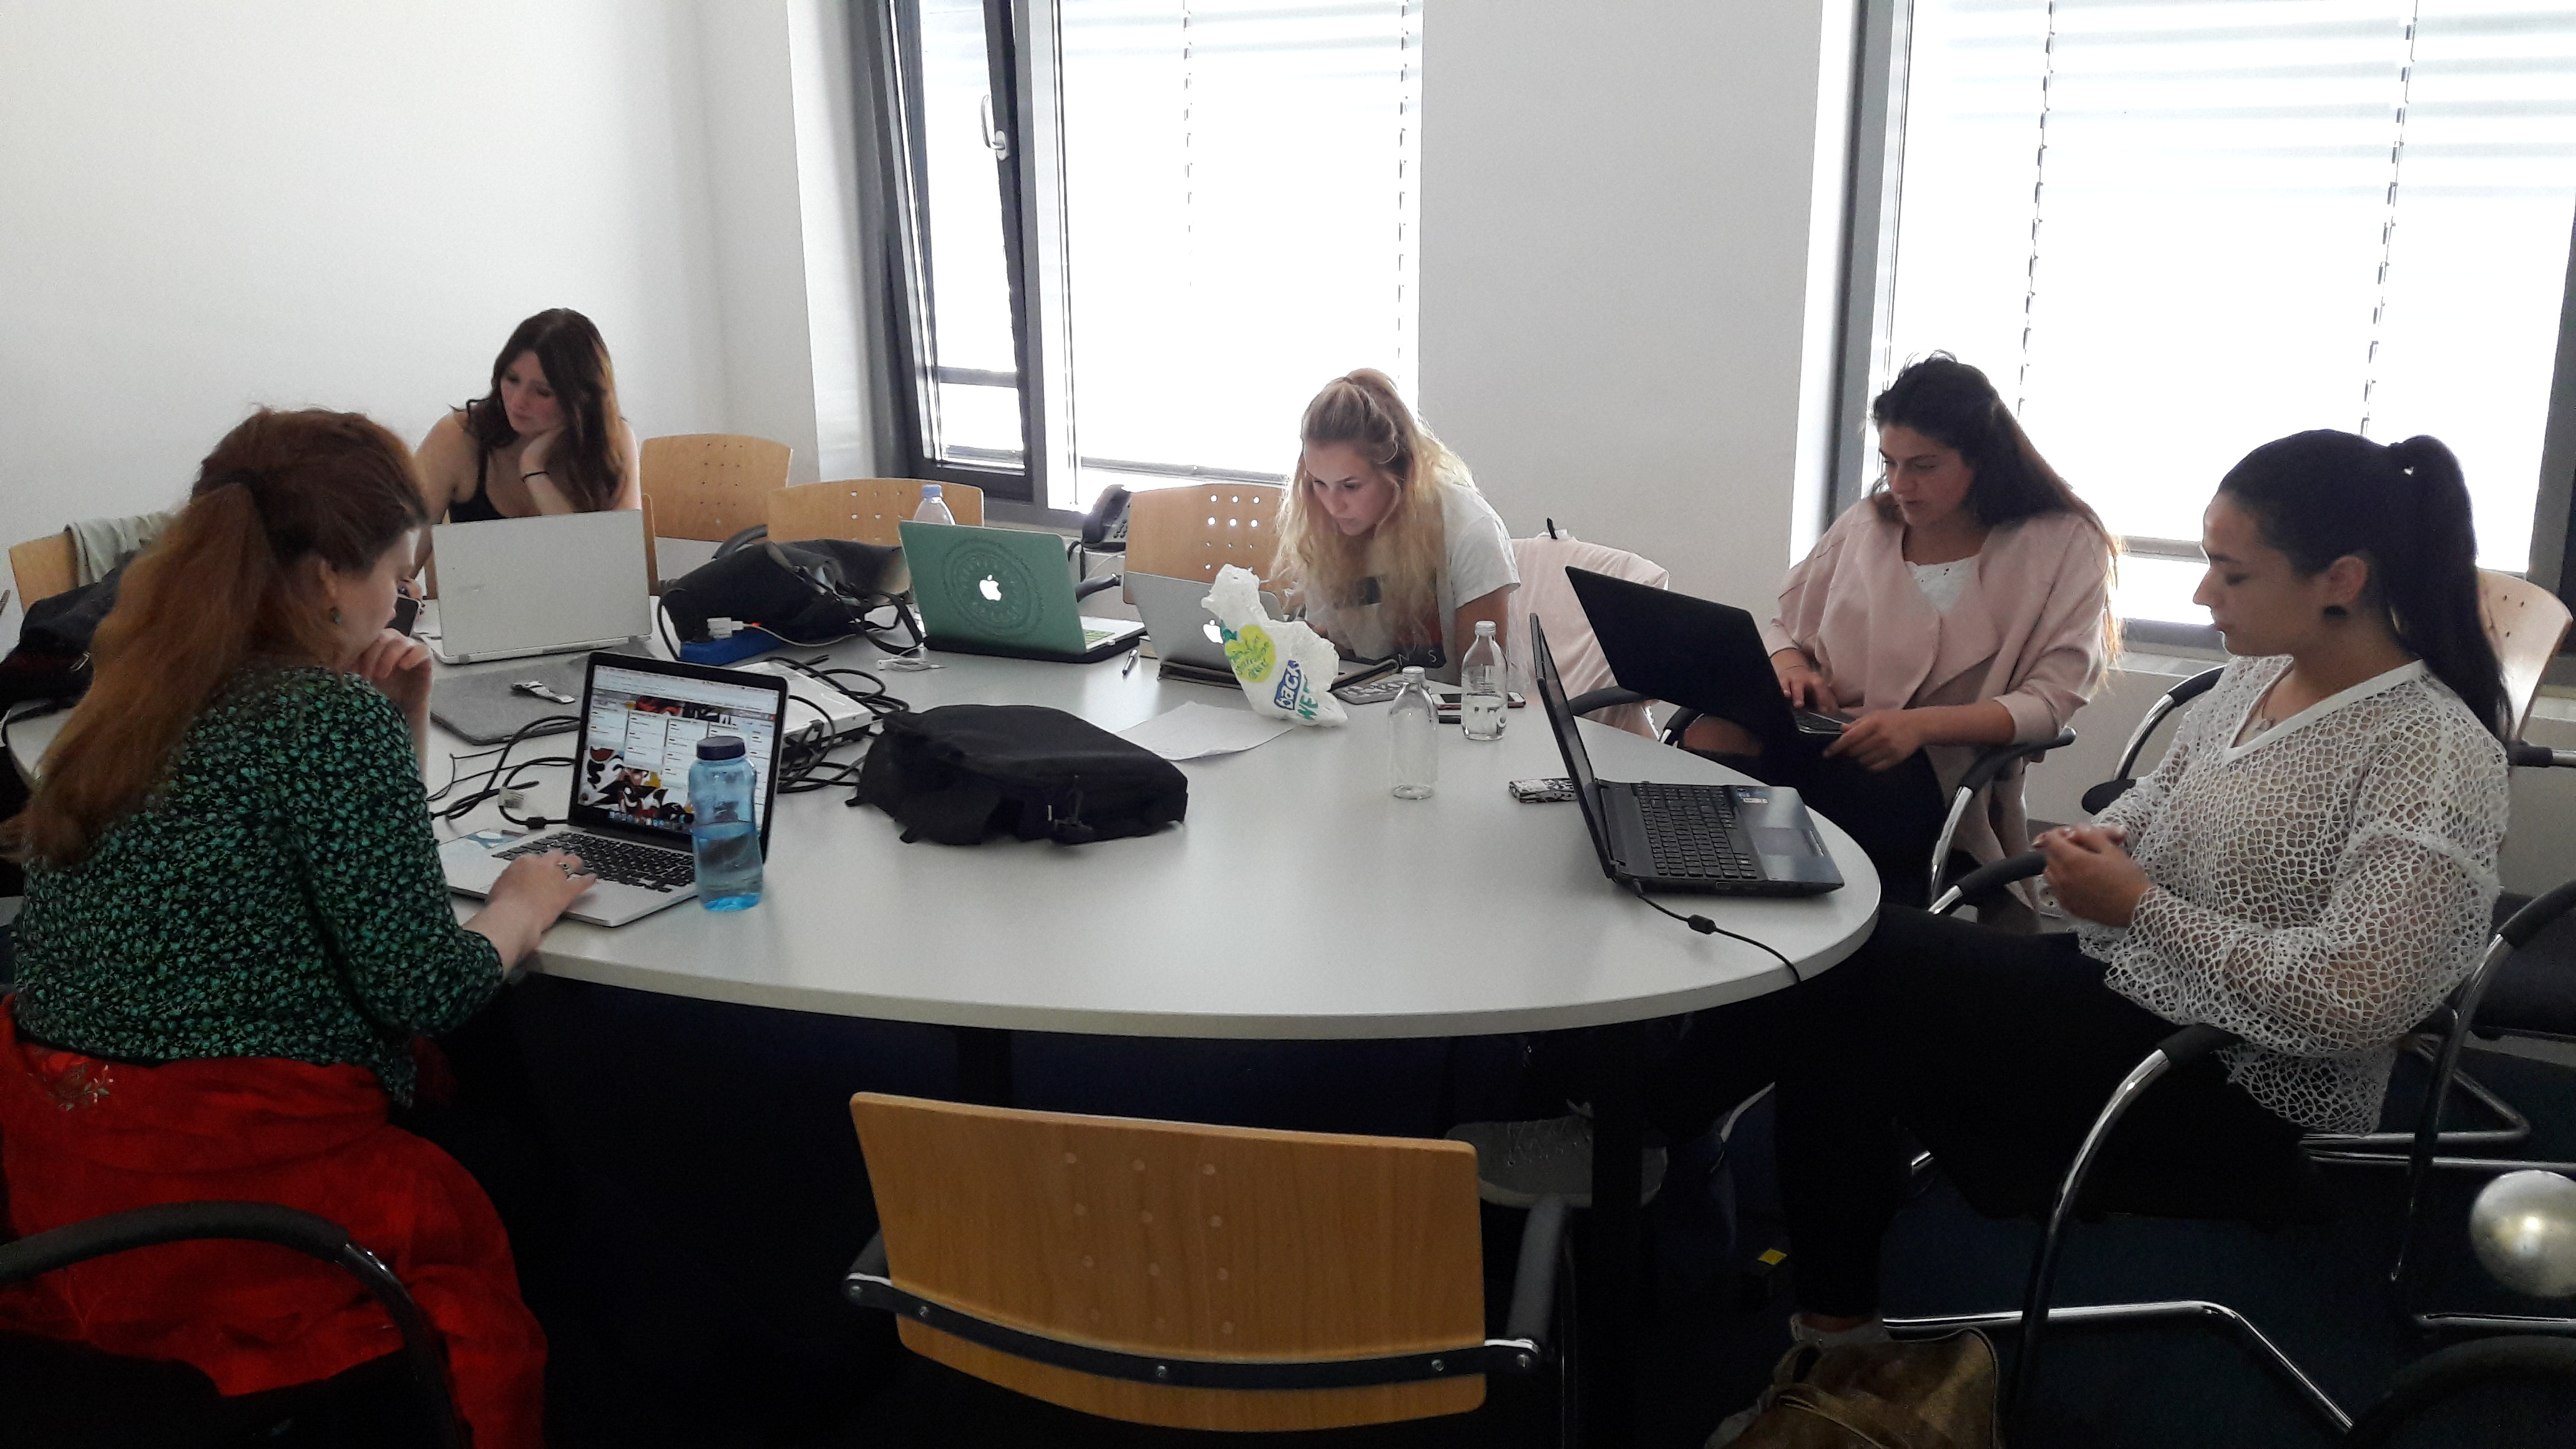
\includegraphics[width=\linewidth, height=\textheight, keepaspectratio]{Bilder/20170518_103125.jpg}
			\caption{Das ¡Experiment!-Team bei der Arbeit}
			\label{img:experiment-team-bei-der-arbeit}
		\end{figure}

		Die Welt war zuerst als recht große Welt geplant, in der man sich frei bewegen kann. Hier sollte man sich viele verschiedene interessante Dinge angucken können und frei durch die Gegend laufen. Hierbei stießen wir jedoch auf das Problem, dass verschiedene Versuchspersonen verschiedene Wege gehen würden und somit unterschiedliche Dinge erleben und manche Szenarien vielleicht sogar komplett auslassen würden. Um dies zu verhindern, kam uns die Idee eier Art Schnitzeljakt. Damit wäre gewährleistet gewesen, dass jeder Versuchsperson ungefähr die gleiche Strecke läuft und das gleiche erlebt wie alle anderen. Jedoch stellte sich auch das als nicht sehr praktikabel heraus. Wir benötigten ein Mapdesign, in dem jede Versuchsperson die gleiche Strecke läuft und das gleiche erlebt.

		So kamen wir darauf, die Versuchspersonen auf einem Gehweg entlanglaufen zu lassen, auf dem es keine betretbaren Abzweigungen gibt und jeder an mehreren Ampeln für eine vordefinierte Zeit warten muss. 
		
		Während des gesamten Designprozesses kam es immer wieder zu Schwierigkeiten und Problemen.
		
		\subsubsection{Blender}
			Blender ist ein sehr komplexes und umfangreiches Programm, dementsprechend hatte jeder von uns eine längere Einarbeitungsphase. Bei kleineren Problemen haben wir uns gegenseitig viel helfen können und unser angesammeltes Wissen ausgetauscht. Die größten Probleme entstanden hauptsächlich nach dem Import in die Unreal Engine. 
%			Normale
%			Texturen
			
			Ein zentrales Problem war, dass jegliche von uns erstellten Objekte nach eine Build des Lightnings komplett schwarz waren. Nach einiger Recherche stellte sich heraus, dass alle in der Unreal Engine verwendeten Objekte zwei UV-Maps benötigen. Die zweite ist notwendig für das korrekte Darstellen des Lightning und ist, zumindest bei statischen Objekten, zwingend notwendig. Sich bewegende Objekte wie beispielsweise die Autos werden anders gerendert und benötigen diese zweite UV-Map nicht. 
		
		\subsubsection{Unreal}
		
		\subsubsection{Hardware}
		
%		Probleme
%			Blender
%			Unreal
%			Controler
%			Kugel
%			Oculus
%			PC-Wechsel
%			Fahrrad
%			Teleport

	\subsection{Versuchsdurchführung} % Daniel
	\subsection{Auswertung} % Marvin
	
%Auswertung
Das Projekt abschließend folgte nach dem 26.03.2017, dem letzten Tag der Versuchsdurchführung, die Auswertung unserer Ergebnisse.
Zunächst mussten wir auch in dieser Phase einige zusätzliche Recherche, vor allem zu mathematischen Verfahren für statistische Auswertung, betreiben. Ebenfalls sehr wichtig waren für uns die genauen Richtlinien zur Veröffentlichung eines wissenschaftlichen Papers. Hierzu erhalten wir ein maßgebendes Buch von unseren Dozenten. Wir unterteilten den Inhalt des Papers und dieses Berichts und teilten diese untereinander auf.\\
Danach begannen wir zunächst damit sämtliche Ergebnisse zu digitalisieren.\\
\\

\section{Versuchsaufbau und Durchführung}
	\todo[inline]{Autor: Nizan}
	\subsection{Probanden}
	Für die Durchführung des Experiments haben wir Probanden benötigt, die als Versuchspersonen
(Abkürzung VP) für die Untersuchung und Überprüfung unserer Forschungsfrage dienen.
Die Versuchspersonen waren bezüglich der experimentellen Hypothese unwissend und unterschrieben
vor der Teilnahme eine schriftliche Einverständniserklärung mit allen Risiken und Datenschutz-
rechtlichen Informationen. Alle Probanden haben freiwillig am Experiment teilgenommen
und wurden nicht entschädigt.
\subsubsection{Demografische Angaben}
Bei der Suche nach Probanden haben wir uns auf Probanden im Alter von minimal 18 Jahren
und maximal 80 Jahren beschränkt, da die Zeitwahrnehmung von Jungendlichen langsamer ist
als die von Erwachsenen. Der Grund: Je mehr Neues und Emotionales man erlebt, desto mehr
prägt sich im Gedächtnis ein; und desto länger wirkt ein Zeitraum im Nachhinein. Das ergab
die Studie „Age effects in perception of time“ von Marc Wittmann und Sandra Lehnhoff aus
dem Jahre 2005. Weshalb wir ausschließlich Erwachsene Probanden gesucht haben, die über
dem Zeitraum der „erste Male erleben“ hinaus sind. Der Mittelwert aller Probanden liegt bei 31
Jahren, ob diese bereits vorher in einer VR waren, haben wir nicht berücksichtigt.
Insgesamt wurden 48 gültige Ergebnisse für die Auswertung benötigt, weshalb wir 50 Probanden
eingeladen haben um am Experiment teilzunehmen, für mögliche Ausfälle, die auch aufgetreten
sind.
Die Verteilung der Geschlechter haben wir offen gelassen, da in dem Ausmaß unseres Experiments
keine signifikanten Unterschiede zustande gekommen wären, das gilt auch für den Bildungsstand
und die Rasse der Probanden. Die Sprachkenntnisse waren uns dennoch wichtig,
aufgrund des Mehrfach-Wortschatz Intelligenztests der auf guten Deutschkenntnissen basiert
und wir die selben Voraussetzungen bei allen Versuchspersonen gewährleisten wollten. Weitere
Voraussetzungen waren eine gute oder auf normal korrigierte Sehkraft durch eine Brille oder
Kontaktlinsen und normales Farbsehen. Außerdem haben wir Versuchspersonen mit Gehirnschäden
oder psychischen Erkrankungen vom Experiment ausgeschlossen, um mögliche Störvariablen
zu verhindern.
\subsubsection{Probanden Suche}
Um die Probanden Suche hat sich das Organisation Team gekümmert. Es wurde eine Projekt EMail
Adresse erstellt, für die Kommunikation und Interaktion zwischen Versuchsleitern und Versuchspersonen.
Die Suche verlief auf drei unterschiedlichen Wegen: (1) Bekannte anwerben,
(2) Flyer Verteilung, (3) Anzeigen auf Sozialen Netzwerken und öffentlichen Portalen veröffentlichen.
In vorher eingeteilten sogenannten „Terminslots“, im Zeitraum von sechs Tagen, wurden
die Probanden eigetragen. Die effektivste Methode Probanden zu finden waren Anzeigen auf
der Website „Ebay-Kleinanzeigen“ zu schalten. Diese wurden mehrmals in der Woche von neuem
geschaltet, sodass eine Großzahl von Menschen die Anzeige lesen konnte, um sich dann bei
uns per Mail zu melden.
Die zweit erfolgreichste Methode Probanden zu finden war im Bekanntenkreis passende Probanden
anzuwerben. Dabei haben wir im Vorhinein die Grenze gesetzt, keine direkten Verwanden,
wie Eltern, Geschwister oder Lebenspartner zu nehmen, da sie eventuelles Vorwissen haben,
was das Ergebnis verfälschen könnte.
Die Methode mit den Flyer hat am schlechtesten funktioniert, da wir die wenigsten Rückmeldung
bekommen haben, was uns gezeigt hat, dass diese Methode etwas veraltet ist.
\par
\underline{Anzeigen Text für Ebay Kleinanzeigen und die Flyer:}
\par
Freiwillige Probanden für VR Experiment gesucht
\par
Bist du im Alter zwischen 18 und 80, bist fit und hast Lust mal in eine Virtuelle Welt einzutauchen?
Dann bist du genau die richtige Person um an unserem Experiment teilzunehmen!
Wir sind eine Gruppe Studenten aus dem Bereich Digitale Medien von der Universität Bremen und
führen im Rahmen unseres Bachelor-Projekts eine Untersuchung zur Wahrnehmung in der virtuellen
Realität. Mit einer VR Brille schicken wir dich in eine andere Welt in der du verschiedene Szenarien
auf dich einwirken lässt.
\par
Wenn du Interesse hast uns bei unserem Experiment zu unterstützen, dann würden wir uns über
eine Email von dir freuen. Nenne uns bitte in deiner Nachricht deinen Namen, Alter, Geschlecht
sowie die Tage an denen du zur Verfügung stehst für das VR Experiment - an folgende Adresse:
experiment.sose17@gmail.com
Unser Experiment werden wir an diesen 6 Terminen durchführen:
Mo 19., Mi 21., Do 22., Fr 23., Sa 24. und Mo 26. Juni 2017 immer jeweils zwischen 10 und 18 Uhr,
im Cartesium an der Universität Bremen. Die Dauer wird 30 Minuten bis 45 Minuten betragen.
Wir freuen uns auf hoffentlich zahlreiche Nachrichten!
\subsubsection{Ethik}
Die Untersuchung menschlichen Verhaltens mit dem Ziel an Forschungsergebnissen zu gelangen,
ist immer etwas problematisch. Besonders, wenn die Manipulation im Rahmen eines Experiments
die Persönlichkeit eines Menschen langfristig prägen oder beeinflussen könnte. Das
zeigte sich uns schon zu Beginn des Projekts, bei der Frage zum Hauptthema des Experiments.
Dabei haben wir unbewusst Themen verworfen, aufgrund der ethischen Moralfrage. Obwohl
einige Vorschläge wirklich interessant waren, hat uns unser gesundes „moralisches Ich“ gesagt,
dass wir diese Ideen als Experiment keinem Probanden zumuten können. Diese hätten
Grenzen überschritten, deren Folgen wir nicht verantworten wollten. Auch wenn es anfänglich
unbewusst geschah und wir uns erst später mit der Frage ethischen Vertretbarkeit beschäftigten,
haben wir uns stets an die moralischen Richtlinien gehalten. Die hohe Nachfrage der freiwilligen
Probanden hat uns gezeigt, dass uns der Spagat zwischen Ethik und einem Experiment
das menschliches Verhalten testet, gut gelungen ist. Uns war wichtig die Sicherheit der Probanden
zu gewährleisten, weshalb sie weitestgehend über Zweck und Ablauf des Verfahrens
sowie über die vorhersehbaren Unannehmlichkeiten und Risiken vorab informiert wurden. Es
wurde vor der Teilnahme eine schriftliche Einverständniserklärung unterschrieben, womit die Probanden die persönliche Verantwortung übernahmen und somit auch die Risiken in kauf
nahmen. Des weiteren haben wir die Versuchspersonen immer ermutigt fragen zu stellen,
wenn welche offen waren, um Zweifel oder Missverständnisse zu vermeiden. Zuletzt werde alle
Ergebnisse und untersuchten Daten streng vertraulich behandelt und anonymisiert nach den
allgemeinen Datenschutzrichtlinien.
\subsection{Apparaturen}
Zwei Räume wurden für die Durchführungen des Experiments genutzt und von uns ausgerichtet.
In Raum 1, haben wir die Fragebögen ausfüllen lassen und die Zeit-Einschätzungs-Tests
durchgeführt. Dort stand ein Tisch und auf den sich gegenüberliegenden Seiten zwei Stühle.
Auf einem separaten Tisch, hinter dem Stuhl der Versuchsleiter, lagen alle benötigten Unterlagen
und Werkzeuge: die Ergebnisse der vergangenen Probanden, der Infrarot-Thermometer
[„Braun ThermoScan 7 Infrarot Ohrthermometer IRT6520“] sowie die dazugehörigen Schutzkappen
- die nach jedem Durchlauf ausgewechselt wurden, ein iPhone 6 zum stoppen der Zeit
und die leeren Fragebögen: (1) Einverständniserklärung, (2) „Fragebogen B“, (3) „Fragebogen
A“, (4) Mehrfach-Wortschatz-Intelligenztest und (5) „Fragebogen C“ (weitere Erläuterungen
unter dem Punkt 5.3.A) Diese haben wir der Reihenfolge nach in Klemmbrettern geordnet und
für die Durchläufe mit den nächsten Versuchspersonen vorbereitet.
In Raum 2 haben wir die praktischen VR-Experimente durchgeführt. Dort stand ein Drehstuhl
um sich flexibel in der Welt bewegen und drehen zu können, ein Tisch mit einem LG Computer
auf dem Windows 10 installiert war und zwei Monitore [Fujitsu Siemens P19-1A \& 2. Benq
FP222WH] auf denen man die virtuelle Welt sehen und mit Unity bearbeiten konnte. Außerdem
war der Raum mit Kopfhörern ausgestattet um äußere Geräusche zu minimieren sowie und die
Audio und Hintergrundgeräusche in der virtuellen Welt zu demonstrieren; die Occulus DK2 VRBrille
zur Orientierung in der VR und ein XBox-Controller für die Steuerung in der Welt.
\subsection{Experiment Ablauf}
Der Zeitraum der Experiment Durchführung lag bei sechs Tagen, in denen jeweils im Durchschnitt
8.3 Versuchspersonen an der Untersuchung teilnahmen. Jeder Durchlauf dauert je nach
Proband zwischen 25 Minuten bis 40 Minuten.
\par
Der Ablauf des Experiments bestand aus drei Teilen. Der theoretische Teil vor der VR, der praktische
Teil in der VR, und der theoretische Teil nach der VR. Die Messmethode war aussagekräftig,
da alle Durchläufe sowie die dazugehörigen Erklärungen bei allen Probanden exakt
gleich stattgefunden haben.
\par
\underline{Teil 1.:}
Jeden Durchgang haben wir mit einer Einweisung durch die Räumlichkeiten begonnen. Der erste
Teil, der theoretische Teil des Experiments findet in unserem Befragungsraum, „Raum 1“
statt. Es sind immer zwei Versuchsleiter (VL) die den ersten Teil des Versuchs durchführen und
dem Probanden gegenüber am Tisch sitzen. Die Arbeit wird geteilt, dass einer VL den Ablauf
leitet und der zweite VL die Ergebnisse notiert und auf Fehler achtet. Alle Ergebnisse der Zeiteinschätzungen
und die Körpertemperatur werden von dem VL auf dem vorgedruckten „Fragebogen
B“ notiert. Die Versuchsperson bekommt keine Einsicht auf ihre Ergebnisse, alle Daten
werden verdeckt aufgeschrieben.
Wir händigen dem Proband eine Einverständniserklärung die er unterschreiben muss:
„Als erstes bekommen Sie eine Einverständniserklärung zur freiwilligen Teilnahme am Experiment,
die sie unterschreiben müssen. Bitte lesen Sie diese gründlich durch. Sollten Sie Fragen
haben, werden wir diese gerne beantworten.“
\par
Als nächstes wird ein Zeit-Einschätzungs-Test durchgeführt, in dem der Proband 40 Sekunden
einschätzen soll, ohne Hilfsmittel und ohne sich zu unterhalten:
„Wir werden nun einen Zeit-Einschätzungs-Test durchführen, indem Sie 40 Sekunden einschätzen
sollen. Dabei dürfen Sie sich nicht unterhalten und sollten Sie eine Armbanduhr tragen,
bitten wir Sie diese abzunehmen. Bei „Los“ geht es los und wenn Sie das Gefühl haben,
dass 40 Sekunden vergangen sind, sagen Sie bitte „Stop““. Das Ergebnis wird von einem VL
notiert.
\par
Das Ergebnis wird von einem der anwesenden VL anhand einer Stoppuhr gemessen und auf
dem „Fragebogen B“ erfasst. Der Proband bekommt den „Fragebogen A“ ausgehändigt:
,,Wir bitten Sie diesen Fragebogen einmal auszufüllen“
Dort sollen folgende Informationen angegeben werden: (1) ob die zu testende Person unter
Drogeneinfluss steht, (2) wie der akute müdigkeitswert ist, (3) ob und an welchen Gehirnschäden
oder psychischen Erkrankungen der Proband leidet , (4) welche die Muttersprache der Versuchsperson
ist und ob die VP noch Lust hat am Experiment teilzunehmen. Wird das Kästchen
mit “Ja“ beantwortet, geht es weiter mit den Tests.
\par
Daraufhin wird der „Mehrfachwahl-Wortschatz-Intelligenztest“ (MWT-B) durchgeführt (weitere
Erläuterungen bei 5.3.B).
\par
„Sie sehen hier mehrere Reihen mit Wörtern. In jeder Reihe steht höchstens ein Wort, das Ihnen
vielleicht bekannt ist. Wenn Sie es gefunden haben, streichen Sie es bitte durch.
Es gibt keine zeitliche Begrenzung also können Sie sich ruhig Zeit lassen. Sollten Sie ein Wort
nicht kennen, dann raten Sie bitte.“ Der ausgefüllte Test wird von den VL entgegengenommen
und ein erneuter Zeit-Einschätzungs-Test wird durchgeführt.
\par
„Wir werden nun erneut einen Zeit-Einschätzungs-Test durchführen, indem Sie 40 Sekunden
einschätzen sollen. Dieses Mal werden wir uns mit Ihnen währenddessen unterhalten. Sie dürfen
sich und uns gerne unterbrechen, wenn Sie das Gefühl haben, die 40 Sekunden sind vorüber.“
Das Ergebnis wird von einem VL notiert.
\par
Anschließend messen wir die Körpertemperatur am Ohr des Probanden, anhand unseres Infrarot-
Thermometers. „Wir werden nun Ihre Körpertemperatur mit diesem Infrarot Thermometer
messen.“ Ein neuer Aufsatz wird auf den Kopf des Thermometers gesetzt und dem Probanden
ins Ohr gehalten „Achtung, nicht erschrecken“. Das Ergebnis wird von einem VL notiert.
\par
Danach führen wir einen stummen 30 Sekunden Zeit-Einschätzungs-Test. „Es wird nun erneut
einen Zeit-Einschätzungs-Test durchgeführt, diesmal sollen Sie lediglich 30 Sekunden einschätzen
ohne sich zu unterhalten. Und Los!“
\par
\underline{Teil 2.:}
Der Proband wird in den isolierten und Schallgeschützen „Raum 2“ geführt, wo der praktische
Teil des Experiment stattfindet. Dort warten die zwei Versuchsleiter von der VR. Währenddessen
werten die ersten beiden VL den Intelligenztest aus.
Der Proband bekommt folgende Anweisung: „Nehmen Sie bitte hier auf dem Drehstuhl platz.
Sie kommen jetzt in unsere virtuelle Welt. Bitte halten Sie sich an die allgemeinen Verkehrsregeln
und prägen Sie sich die Umgebung ein.“
Der Proband setzt sich, bekommt die VR-Brille aufgesetzt und den Xbox Controller in die Hand.
„Die Fortbewegung in der virtuellen Welt wird mittels eines Xbox-Controllers kontrolliert. Mit
der rechten Taste können Sie die Ausrichtung der Kamera ändern, dies tun Sie am besten
wenn Sie an eine Straßenecke gelangen. Ansonsten schauen Sie sich lieber mit der Brille um.
Mit der linken Taste können Sie Vorwärts und Rückwärts gehen, sie dürfen selbst entscheiden
wie schnell oder langsam Sie gehen und sich sonst frei bewegen. Sie können auch gerne zwischendurch
stehen bleiben und sich umschauen wenn Sie wollen.“ Der Proband darf die Steuerung
testen, danach werden ihm vom VL die Kopfhörer aufgesetzt und der Durchlauf in der VR
beginnt.
\par
Zu Beginn des VR Experiments wird die Zeit von einem Versuchsleiter gestoppt, solange wie
der Proband benötigt um die gesamte Strecke der vier Szenarien zu durchlaufen. Erfasst wird
die Zeit vom Zeitpunkt des los Laufens bis zur Ankunft am Schild „Road Closed“. Die vier Szenarien
bilden zusammen die virtuelle Welt und bestehen aus insgesamt vier Ampelphasen. Diese
sind visuell und auditiv einer realen Welt nachgebaut mit Wegen, Straßenverkehr, Autolärm,
Menschen, Häuser und Bäumen. An jeder Ampelphase gibt es einen manipulierten Faktor, der
die Zeitwahrnehmung beeinflusst. Immer zwei der Szenarien gleichen sich optisch, mit dem
Unterschied, dass den Gegenteiligen Faktor haben. Einer schnell, der andere langsam. (a) Ampelphase
an einem LKW - schnelles Ticken, (b) Ampel mit Vogel und Menschen - langsames
Ticken, (c) Ampel neben einem schaukelndem Kind mit rosa Shirt - schnelles schaukeln, (d)
Ampel mit Heißluftballon-Plakat bei einem schaukelndem Kind mit grünem Shirt - langsames
Schaukeln.
\par
Die Wartezeit an den Ampeln ist von uns vorgegeben und kann nicht frühzeitig übersprungen
werden. Der Proband durchläuft die virtuelle Welt ein mal, ohne Pausen in seinem eigenen
Tempo. Die Versuchsleiter beobachten das Verhalten des Probanden in der VR mittels von Bildschirmen
und können eingreifen, sollte etwas schiefgehen. Nach Beendigung des Laufs, wird
dem Probanden die Brille sowie die Kopfhörer wieder abgesetzt und dieser begibt sich zurück in
„Raum 1“, für den letzten Theorieteil.
\par
\underline{Teil 3.:}
Der Proband nimmt erneut platz am Tisch, gegenüber von den Versuchsleitern.
Es werden 40 Sekunden ohne Unterhaltung abgeschätzt und vom Versuchsleiter notiert. Die
Anweisungen in Teil 3., bleiben die gleichen wie in Teil 1.
Der Proband erhält den „Fragebogen C“, den dieser mit diesen Informationen ausfüllen soll:
(1) die geschätzte Dauer von den einzelnen Szenarien (2), die besten und schlechtesten empfundenen
Szenarien, (3) die empfundene Dauer in der virtuellen Welt, (4) den eigens empfundenen Spaßfaktor, (5) auffallende Besonderheiten in der virtuellen Welt und (6) eine Einschätzung
worum es in dem Experiment ging.
Ein erneuter Zeit-Einschätzungs-Test wird durchgeführt, in dem die Versuchsperson 40 Sekunden
abschätzen und sich gleichzeitig mit einem der Versuchsleiter unterhalten soll. Die Ergebnisse
werden von den Versuchsleitern notiert. Zum Schluss findet ein 30 Sekunden Zeit-Einschätzungs-
Test ohne reden statt. Das Experiment wird danach beendet. Der Proband darf anschließend
seine Zeit-Einschätzungs-Ergebnisse erfahren sowie das Ergebnis vom Intelligenztest.
Zum Schluss wird der Proband verabschiedet und der nächste Proband vom Treffpunkt
abgeholt.
\subsubsection{Fragebögen}
Wir haben uns um unsere Evaluationsdaten zu sammeln für das Verfahren des Fragebogens
entschieden. Mit dieser Methode kann man ohne viel Aufwand zu vielen Informationen gelangen,
auf die man auch zu späteren Zeitpunkten zurückgreifen kann, da Fragebögen reproduzierbar
sind. Sie ermöglichen die Objektivität der Befragung und es wird sichergestellt, dass
jede Versuchsperson die exakt selben Fragen beantworten muss. Diese Methode benötigt einen
geringeren Personalbedarf gegenüber dem Interview und bietet zudem noch einen Organisationsvorteil,
da die Prozedur schneller und flächendeckender abläuft. Durch die Anonymität des
Befragten, ist dieser beim ausfüllen des Fragebogens weniger gehemmt und beantwortet die
Fragen automatisch ehrlicher aber auch sorgfältiger, weil kein Zeitdruck besteht schnell antworten
zu müssen.
\par
\underline{Bezug auf „Fragebogen A“:}
In Fragebogen A wurde der körperliche und psychische Zustand des Probanden abgefragt um
mögliche Beeinträchtigungseinflüsse zu kennen.
1. Stehen Sie unter irgendwelchen Drogeneinflüssen oder Medikamenten?
Da Drogen jeglicher Art und manche Medikamente die die Wahrnehmung beeinflussen und bei
Einfluss dieser Substanzen die Ergebnisse nicht verwendbar wären, haben wir die Probanden
nach dieser Information abgefragt.
2. Auf einer Skala von 1 bis 10, wie müde sind Sie? (1 = nicht müde - 10 = sehr müde)
Eine sehr hohe Müdigkeit mindert die Konzentrationsfähigkeit. Bei einem Müdigkeitswert ab 8
ist die Messung unter Vorbehalt verwendbar und deshalb auch relevant für unsere End Ergebnisauswertung.
3. Haben Sie Ihnen bekannte Gehirnschäden oder psychische Erkrankungen?
Probanden mit Gehirnschäden und psychischen Erkrankungen würden möglicherweise zu einem
verfälschtem Ergebnis führen, weshalb die Probanden nach Erkrankungen abgefragt wurden.
4. Ist Deutsch ihre Muttersprache? Wenn Nein, welche Sprache ist ihre Muttersprache?
Die Deutschkenntnisse unserer Probanden waren uns aufgrund des Intelligenztest, der auf der
deutschen Sprache basiert wichtig, um alle Probanden auf dem selben Niveau testen zu können.
5. Möchten Sie das Experiment weiterhin durchführen?
Dem Probanden wurde die Möglichkeit gegeben das Experiment vorzeitig zu beenden.
\par
\underline{Bezug auf „Fragebogen B“:}
Dieser Fragebogen diente lediglich den Versuchsleitern als zweck die Ergebnisse der Zeiteinschätzungen
und Körpertemperatur auf Papier zu bringen in einer Form die reproduzierbar und
geordnet ist.
\par
\underline{Bezug auf „Fragebogen C“:}
1. Sortieren der Szenarien / Ampelphasen vom kürzesten zum längsten mit Sekundenangabe
Die Wahrnehmung der einzelnen von uns beeinflussten Szenarien mittels Gravitationsfaktoren
und Auditiven Einflüssen. Durch die Anordnung der Szenarien nach der Zeit zeigt sich wie sehr
wir die Wahrnehmung der Versuchspersonen beeinflussen konnten.
2. Sortieren der Szenarien vom besten zum schlechtesten
Wir wollen schauen ob das optische empfinden den Szenarien gegenüber die Wahrnehmung
der Versuchspersonen beeinflusst hat.
3. Einschätzung der Gesamtdauer in der VR > multiple choice
Das empfinden der Probanden ob die gesamte Zeit in der VR als länger oder kürzer als die tatsächliche
Zeit wahrgenommen wurde, ist für uns ein weiterer Interessantes Ergebnis zur Zeitwahrnehmung
die wir rausfinden wollen.
4. Hatten Sie Spaß?
Beeinflusst der Spaßfaktor das Empfinden in der VR, ganz nach dem Motto „wenn man Spaß
hat vergeht die Zeit am schnellsten“ oder „wenn man was neues entdeckt oder lernt kommt sie
einem länger vor“
5. Besondere Auffälligkeiten
Auffälligkeiten die eine Zeitwahrnehmung beeinflussen könnte und ein Platz für die Probanden
um ein Kommentar zu hinterlassen.
6. Haben Sie entdeckt was wir mit dem Experiment rausfinden wollten?
Abfragung ob das Experiment zu offensichtlich oder gut genug konzipiert war, dass die Probanden
nicht rausgefunden haben was wir testen wollen.
\subsubsection*{Intelligenztest}
Basierend auf der Studie „Zeiterleben in der Tempogesellschaft“ vom Autor Pascal Wallisch aus
der Uni Chicago, in der beschrieben wird, dass die Intelligenz eines Menschen sein Zeiterleben
beeinflusst, haben wir beschlossen einen Intelligenztest in unser Experiment zu integrieren. Bei
einem Treffen mit dem Master Psychologie Studenten Till Rachwitz, der sich auf Intelligenztests
spezialisiert hat, haben wir verschiedene Methoden kennengelernt, wie man die Intelligenz unserer
Probanden testen kann, ohne einen mehrstündigen Test durchführen zu müssen. Dabei
sind wir auf den psychologisch anerkannten „Mehrfach-Wortschatz-Intelligenztest (MWT-B)“ in
der fünften unveränderten Auflage gestoßen, entwickelt von Siegfried Lehre, veröffentlicht im
Jahre 2015, der sehr gut für unser Vorhaben geeignet ist. Dieser bereits langjährig angewandte
Test dienst zur Messung des allgemeinen Intelligenzniveaus nach einem einfachen und zuverlässigen
Schema.
Im MWT-B gilt es aus 37 Wortreihen, bestehend aus jeweils vier erfundenen und einem deutschen
Wort, das richtige Wort rauszusuchen und durchzustreichen. Der Schwierigkeitsgrad
steigt im Laufe des Tests, es beginnt mit Alltagswörter wie „Nase“ und endet mit sehr raren
Worten aus dem deutschen Wortschatz wie „Purin“ Die aktuell verfügbare Leistungsfähigkeit wird anhand dieses Tests mit einem geringen Materialaufwand
gemessen. Die einfache Wiederholbarkeit und die schnelle und einfache Durchführung
innerhalb von circa 5 Minuten, sind zwei der vielen Vorteile dieses Tests für den Zweck
unserer Studie. Zwar spielt die Intelligenz der Probanden in unserem Experiment eine Rolle,
jedoch nur eine nebenläufige, sodass wir nicht viel Zeit dafür einplanen wollten wie bei einem
Standard Intelligenztest. Ein weiterer Vorteil des MWT-B, ist dass dieser von Personen durchgeführt
werden kann, die keine spezielle Ausbildung zur Abnahme von IQ-Tests haben. Des
Weiteren ist der Test objektiv, robust und ist weitgehend unabhängig von seelisch-geistigen
Störungen.
Den MWT-B haben wir in der Testothek an der Psychologischen Abteilung der Uni ausleihen
dürfen.
	\subsection{Aufbau \& Apparaturen}
	\subsection{Experiment Ablauf}
	\subsubsection{Fragebögen}
	\subsubsection{Intelligenztest}
	\subsubsection{Genaue Wortlaute bei der Testphase}
	\subsubsection{Schwierigkeiten}
	\subsection{Ethik}

\section{Beobachtungen}
	\todo[inline]{Autor: Nicole \& Svenja}
	Nur Verweis auf Paper!

\section{Auswertung}
	\todo[inline]{Autor: Nicole \& Svenja}
	Nur Verweis auf Paper!

\section{Interpretation}
	\todo[inline]{Autor: Nicole \& Svenja}
	Nur Verweis auf Paper!
	
\section{Fazit}
	\todo[inline]{Autor: Chovi}

	Zusammenfassung: Was wurde grob in dieser Arbeit gemacht? Was waren die Schlüsselergebnisse?

	Wem nützen die Beiträge der Arbeit? Inwieweit wird die Wissenschaft durch die Arbeit verbessert?

	Aufbauende Arbeiten: Welche möglichen Lösungsansätze für noch bestehende Probleme sind denkbar(mehr Probanden)? Wie könnten Folgearbeiten aussehen?

\section{Abschließende Gedanken}
	\todo[inline]{Autor: Jana}
	Wir sind in den verschiedenen Phasen des Projekts auf unterschiedliche Probleme gestoßen, von denen wir viele zeitnah lösen konnten. Allerdings gab es auch schwerwiegendere, deren Lösung für uns nicht gleich oder gar nicht offensichtlich war und die unseren ursprünglichen Zeitplan infolgedessen ungewollt stark beeinflusst haben.\\
	Eines der größten Hindernisse in unserem Projekt waren technische Probleme, die ein Vorankommen sehr stark verzögerten und in einem veränderten Zeitplan resultierten.\\
	Durch die Inkompabilität der Ocolus Rift und dem Computer der Virtusphere konnten wir unser Projekt nicht wie ursprünglich geplant in der Virtusphere stattfinden lassen und mussten auf herkömmliche Controller ausweichen. Diese Umstellung ist sehr ärgerlich, da viel Zeit in die Problemlösung investiert wurde und wir den Probanden letztendlich doch nicht das bieten konnten, mit dem wir sie ursprünglich geworben haben. 
	Weiterhin zu kritisieren wäre eine nicht ganz ideale Arbeitsteilung, wodurch es gerade am Ende zu erheblichem Zeitverzug kam. Insbesondere das sog. \textit{Technikteam}, welches primär für die Erstellung der Blenderobjekte, das Einsetzen und das Animieren der Welt verantwortlich war, hat gleich zu Beginn des Projekts anstehende Aufgaben nicht sinnvoll verteilt. Alle Mitglieder waren gleichermaßen nur mit \textit{aktuellen} Aufgaben beschäftigt. D.h., dass zunächst alle für die Erstellung von Blenderobjekten verantwortlich waren und so Kapazitäten und Zeit verschwendet wurde, da sich bisher noch keiner besonders gut mit der Software auskannte und sich alle gleichermaßen neu einarbeiten mussten.\\
	Diese Entscheidung mag daraus resultieren, dass wir im Bezug auf so eine Art von selbstorganisierter Arbeit sehr unerfahren sind und es dadurch zu Fehleinschätzungen kam.\\
	Im Nachhinein stellen wir weiterhin fest, dass es für das Projekt besser gewesen wäre, hätten wir zu Beginn andere Prioritäten festgelegt. Da die Logik der Welt der Punkt ist, von dem die Ergebnisse abhängen, hätte man sich zuallererst auch mit dieser beschäftigen müssen bzw. rechtzeitig die Personen bestimmen müssen, die die Hauptverantwortung für diese übernehmen.\\
	Auch diese Fehleinschätzung zeigte sich im Nachhinein als kritisch.

\section{Appendix} % = Anhang
	\todo[inline]{Autor: Alina}
	Anhang.
	
\vfill %Zum Seitenende Verschieben

\printbibliography

\end{document}
